\documentclass[a4paper]{article}
    \usepackage[pdftex]{hyperref}
    \usepackage[latin1]{inputenc}
    \usepackage[english]{babel}
    \usepackage{a4wide}
    \usepackage{amsmath}
    \usepackage{amssymb}
    \usepackage{algorithmic}
    \usepackage{algorithm}
    \usepackage{ifthen}
    \usepackage{listings}
    % move the asterisk at the right position
    \lstset{basicstyle=\ttfamily,tabsize=4,literate={*}{${}^*{}$}1}
    %\lstset{language=C,basicstyle=\ttfamily}
    \usepackage{moreverb}
    \usepackage{palatino}
    \usepackage{multicol}
    \usepackage{tabularx}
    \usepackage{comment}
    \usepackage{verbatim}
    \usepackage{color}
    
    % Because of an error on line 41 I added this
    \usepackage{graphicx}
    
    % Used for drawing DFAs and NFAs
    \usepackage{tikz}
    \usetikzlibrary{automata, positioning}
    
    %% pdflatex?
    \newif\ifpdf
    \ifx\pdfoutput\undefined
    \pdffalse % we are not running PDFLaTeX
    \else
    \pdfoutput=1 % we are running PDFLaTeX
    \pdftrue
    \fi
    %\ifpdf
    %\usepackage[pdftex]{graphicx}
    %\else
    %\usepackage{graphicx}
    %\fi
    \ifpdf
    \DeclareGraphicsExtensions{.pdf, .jpg}
    \else
    \DeclareGraphicsExtensions{.eps, .jpg}
    \fi
    
    \parindent=0cm
    \parskip=0cm
    
    \setlength{\columnseprule}{0.4pt}
    \addtolength{\columnsep}{2pt}
    
    \addtolength{\textheight}{5.5cm}
    \addtolength{\topmargin}{-26mm}
    \pagestyle{empty}
    
    %%
    %% Sheet setup
    %% 
    \newcommand{\coursename}{Formal Languages and Logic}
    \newcommand{\courseno}{CO21-320211}
     
    \newcommand{\sheettitle}{Homework}
    \newcommand{\mytitle}{}
    \newcommand{\mytoday}{\textcolor{blue}{October 03rd}, 2018}
    
    % Current Assignment number
    \newcounter{assignmentno}
    \setcounter{assignmentno}{3}
    
    % Current Problem number, should always start at 1
    \newcounter{problemno}
    \setcounter{problemno}{1}
    
    %%
    %% problem and bonus environment
    %%
    \newcounter{probcalc}
    \newcommand{\exercise}[2]{
      \pagebreak[2]
      \setcounter{probcalc}{#2}
      ~\\
      {\large \textbf{Exercise \textcolor{blue}{\arabic{problemno}}} \hspace{0.2cm}\textit{#1}} \refstepcounter{problemno}\vspace{2pt}\\}
    
    \newcommand{\bonus}[2]{
      \pagebreak[2]
      \setcounter{probcalc}{#2}
      ~\\
      {\large \textbf{Bonus Problem \textcolor{blue}{\arabic{assignmentno}}.\textcolor{blue}{\arabic{problemno}}} \hspace{0.2cm}\textit{#1}} \refstepcounter{problemno}\vspace{2pt}\\}
    
    %% some counters  
    \newcommand{\assignment}{\arabic{assignmentno}}
    
    %% solution  
    \newcommand{\solution}{\pagebreak[2]{\bf Solution:}\\}
    
    %% Hyperref Setup
    \hypersetup{pdftitle={Homework \assignment},
      pdfsubject={\coursename},
      pdfauthor={},
      pdfcreator={},
      pdfkeywords={Formal Languages and Logic},
      %  pdfpagemode={FullScreen},
      %colorlinks=true,
      %bookmarks=true,
      %hyperindex=true,
      bookmarksopen=false,
      bookmarksnumbered=true,
      breaklinks=true,
      %urlcolor=darkblue
      urlbordercolor={0 0 0.7}
    }
    
    \begin{document}
    \coursename \hfill Course: \courseno\\
    Jacobs University Bremen \hfill \mytoday\\
    \textcolor{blue}{Dragi Kamov and Dushan Terzikj}\hfill
    \vspace*{0.3cm}\\
    \begin{center}
    {\Large \sheettitle{} \textcolor{blue}{\assignment}\\}
    \end{center}
    
    \exercise{}{0}
    \solution
    \textcolor{blue}{
    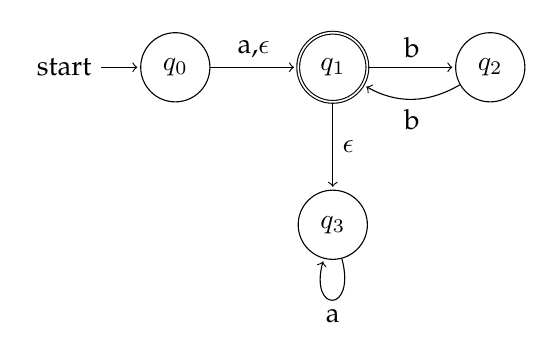
\begin{tikzpicture}[shorten >=1pt, node distance=2cm, on grid, auto]
        \node[state, initial](q0){$q_0$};
        \node[state, accepting](q1)[right=of q0]{$q_1$};
        \node[state](q2)[right=of q1]{$q_2$};
        \node[state](q3)[below=of q1]{$q_3$};
        \path[->]
        (q0)    edge node {a,$\epsilon$} (q1)
        (q1)    edge node {b} (q2)
                edge node {$\epsilon$} (q3)
        (q2)    edge [bend left=30] node {b} (q1)
        (q3)    edge [loop below] node {a} ();
    \end{tikzpicture}}
    
    \exercise{}{0}
    \solution
    \textcolor{blue}{$ (\epsilon + a)b + (\epsilon + a)(b(b + a)a^*)b $}
    
    \exercise{}{0}
    \solution
    \textcolor{blue}{
    The language L presented in the exercise is not a regular language. Here is why: \\ \\
    \textbf{Proof by contradiction (pumping lemma):} Assume L is regular. Given a word $w=1^n0^n$ and $w\in L$, the word $w$ surely has length greater than $n$. According to the lemma, we can split the word in such way $w=xyz$ where:
    \begin{enumerate}
        \item $|y|\neq 0$
        \item $|xy|\le n$
        \item $xy^iz\in L$, for $i>0$
    \end{enumerate}
    Let's say that $y=1^k$, $x=1^l$ and $z=1^{n-l-k}0^n$, where $0<k,l<n$. According to (3) $xy^iz\in L$. If $i=2$, we have the following:
    \begin{equation}
        xyyz=1^l1^{2k}1^{n-k-l}0^n=1^{n+k}0^n \notin L 
    \end{equation}}
    
    \exercise{}{0}
    \solution
    \textcolor{blue}{
    Let us define another language $L^{'}=\{0^{2k+1} | k\ge 0\}$. Since the $L\subseteq L^{'}$, if we proove that $L^{'}$ is not regular, then automatically L is not regular. \\ \\
    \textbf{Proof (pumping lemma):} Assume that $L^{'}$ is a regular language and $w\in L^{'}$ and n is a constant where $|w|\ge n$. Then we can write $w=xyz$ where:
    \begin{enumerate}
        \item $|y|\neq 0$
        \item $|xy|\le n$
        \item $xy^iz\in L$, for $i>0$
    \end{enumerate}
    If $x=0^n$, then one of the following must hold: $y=0^n$ (case 1) or $y=0^1$ (case 2) ($y\neq \epsilon$ because of (2)). For case 1 $z=0^1$ for case 2 $z=0^n$. Let's consider case 2 (the proof for case 1 is the same): consider (3). Then we have:
    \begin{equation}
        0^n0^{k+1}0^n \notin L^{'}
    \end{equation}
    $L^{'}$ is not regular, therefore L is not regular either.}
    
    \newpage
    \exercise{}{0}
    \solution
    \textcolor{blue}{
    $ |v| = n $ \\ 
    That means that: $ |0| + |1| = n $ (in $ v $) \\ 
    Now let's define a homomorphism such that: $ h(0) = 0 $ and $ h(1) = 0 $ \\
    $ h(x_1 ... x_n) = h(1)...h(n) $ \\
    And from that we can transform $ M $ to a language $ N=\{0^n \in \{0\}^*\} $ \\
    From this we can see that $ N $ is equivalent with $ L_{|M|} $, and knowing that $ L_{|M|} $ is a homomorphism of $ M $ and we can conclude that $ M $ is a regular language.}
    
    \exercise{}{0}
    \solution
    \textcolor{blue}{
    \begin{itemize}
        \item[a)] $ L = \{0^n \in \{0\}^* | n>0\}$ with $ \Sigma = \{0\} $ \\ Because if we have only one symbol in our language it is easier to maintain the conditions given in the problem.
        \item[b)] Using the pumping lemma let's represent $ wvvvv... $ as $ wv^kz $, where $ z $ is a sequence that is at the end of this concatenated word. \\ From the conditions of this problem we know that there is only one word of a length and we know that $ L $ is a regular sequence language. And because of this we know that there is only one word $ wv^kz $. The consecutive word would be $ wv^{k+1}z $. As $ k $ would grow all words after $ wv^kz $ are being formed and we could drop the $ z $. \\ By all this we proved that all words in this regular sequence language is represented by $ wvvvv... $
    \end{itemize}}
    
    \end{document}